\section{Miscellaneous Characters}

\subsection*{Delilah Hardstone}

\begin{center}
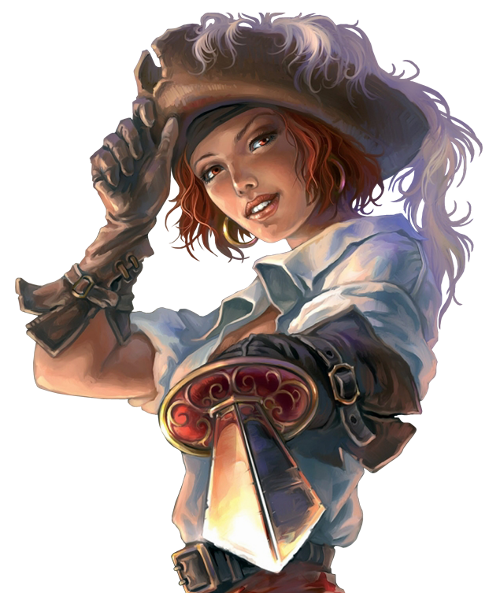
\includegraphics[width=80mm]{./content/img/delilah.png}
\begin{figure}[h]
\end{figure}
\end{center}

\noindent

One of Jennie's Girls, a group confusingly led by a Mae Harkwood!  This hotty was a straight up drop bear killer.  Delilah joined the party during the hunt for Diego Escabar's Fancy Men, quickly proving herself as an expert marksman and fearless fighter.  She shot a rainbow at a shadow creature, helped steal an entire lemon orchard, and flirted with anything that moved, including Gary, who remained oblivious.

Delilah became the Sky Captain of Tomorrow, and then betrothed to Riphard.  The two had twin children together, Bilbo and Dildo, blessed by the gods and believed to possess special powers.  She was killed by Kolo during his rampage in the Hope's Rest sewers, her skull crushed by his monstrous claw.  Her soul went to Hell, confirmed by Lazarus.  Riphard never truly recovered from her death, descending into a delusion that involved a mannequin corpse-wife and two sacks of rotten pork he believed were his children.

\smallskip

\subsection*{Archibald}

\noindent

The elderly, near-blind librarian who continued to tend the abandoned Book Burners headquarters in Hope's Rest long after everyone else had fled.  Archibald lived alone with his son in the building, subsisting on mysterious foodstuffs and maintaining the library with a devotion that bordered on the tragic.  He couldn't see well enough to clean the place properly, but he could still make a decent bacon and eggs.

When the party claimed the building as the Gary Guild's headquarters, Archibald was put to work stripping out the third floor for Exme's workshop, a task he performed with characteristic reluctance.  He developed a surprising romance with Daisuke, the party's Masudan interpreter.

\smallskip

\subsection*{Lazarus}

\begin{center}
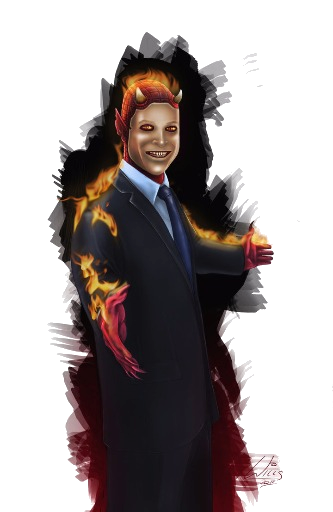
\includegraphics[width=80mm]{./content/img/lazarus.png}
\begin{figure}[h]
\end{figure}
\end{center}

\noindent

A bureaucratic devil in Hell, full name Lazarus ``Laz'' Goldstein.  Lazarus enlisted the help of the group to bring down the Church due to excessive numbers of hell-bound souls caused by the Church's draconian definition of sins.  Red-skinned and wearing a human face mask, Lazarus communicated with the party through their dreams and via the Stone of Unthala.

Despite Kolo's sworn vengeance against him and the group's general distrust, Lazarus proved to be ``a pretty decent bloke'' who had genuinely good intentions, rescuing the party from inevitable deaths he had no part in orchestrating and giving them new leases of life to improve the world.

Following the return of the Gods, Lazarus was rewarded for his efforts by being re-ascended into his full angel form.

\smallskip

\subsection*{Kevin}

\begin{center}
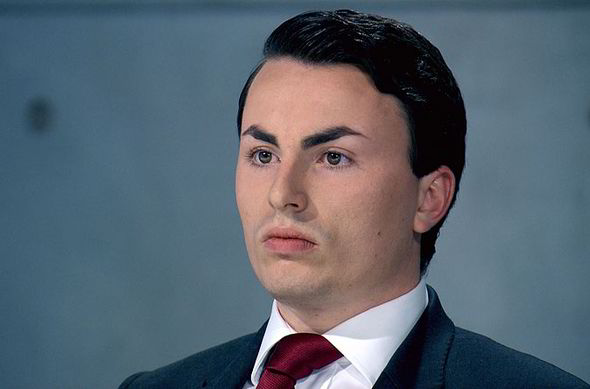
\includegraphics[width=80mm]{./content/img/kevin.jpg}
\begin{figure}[h]
\end{figure}
\end{center}

\noindent

A final-year PhD student at the University of Assassins, Kevin was introduced to the party by Buck McCraw, Burnie's half-Tengu son, as a promising student who needed field experience.  He wrote formal report-letters to ``Professor McCaw'' documenting the group's adventures, and quickly found himself in an ``unhealthily abusive'' mentor-pupil relationship with Burnie.

Kevin possessed a Christopher Mintz-Plasse energy that endeared him to nobody.  Myron threw bottles at his head upon his first boarding of the ship.  His stealth skills, however, proved genuinely useful, he scouted enemy positions, connected with Thieves Guild networks for intelligence, and climbed on a storm giant during the battle for the Bright Bart Forge.  He also substituted gravy for Bovril in Myron's ``Piece of Shit'' cocktails without detection, perhaps his most dangerous accomplishment.

In his spare time Kevin enjoys developing immunity to poisons and fantasy roleplaying games.

\smallskip

\subsection*{Captain Stick}

\begin{center}
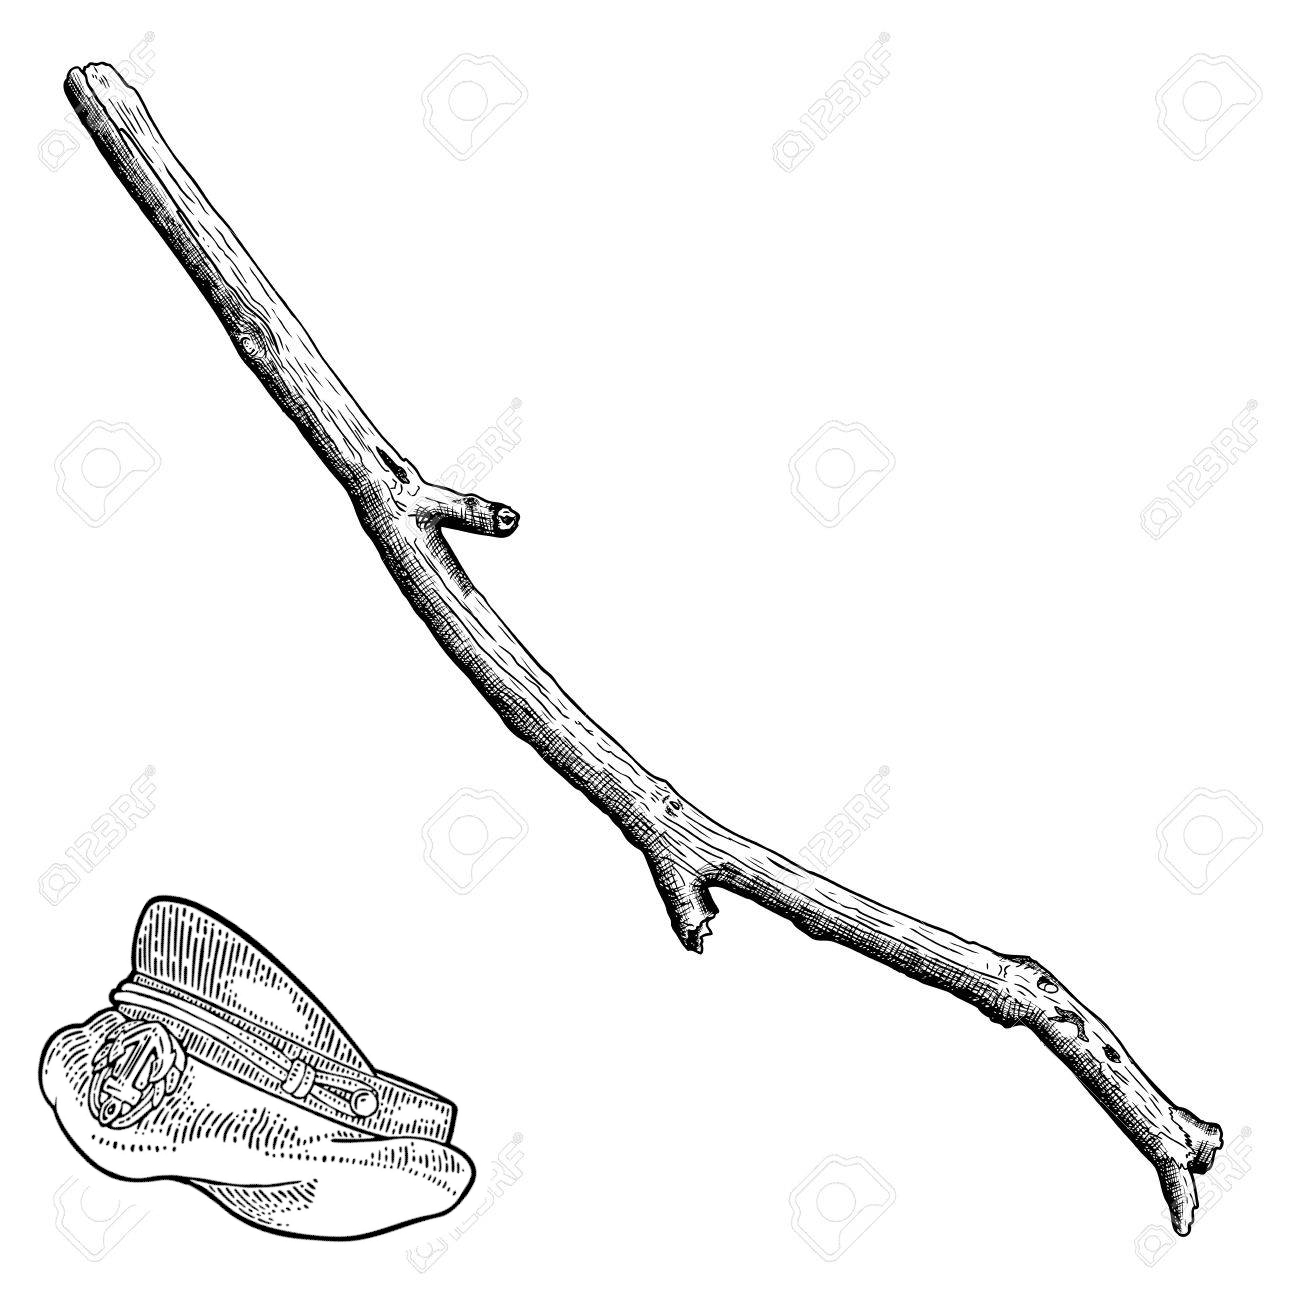
\includegraphics[width=80mm]{./content/img/captainStick.jpg}
\begin{figure}[h]
\end{figure}
\end{center}

\noindent

Not much is known about Captain Stick other than that he has inexplicably been long-trusted with command of The Gary.  Never wavering, seldom faltering in his duties, Captain Stick has offered straight and to-the-point leadership to the team and the airship's crew throughout their adventures.

\smallskip

\subsection*{Vu Dong}

\begin{center}
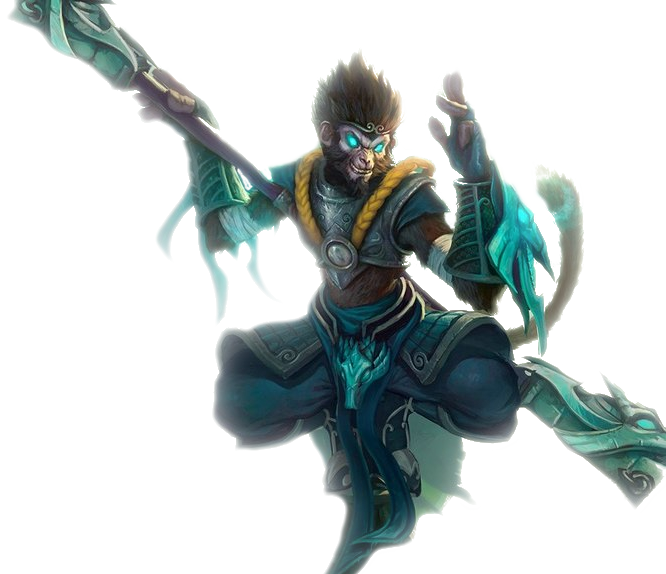
\includegraphics[width=80mm]{./content/img/vu.png}
\begin{figure}[h]
\end{figure}
\end{center}

\noindent

A magical monkey companion who joined the party's menagerie of unlikely allies.  Vu Dong wielded staves and Pilch's old sword with surprising effectiveness, navigating by tail-stick when blinded.  Sometimes called Jeremy or Jezza, the monkey served as mascot, scout, and occasional combatant, though Mark once complained he's ``not really here when we need him''.

\smallskip

\subsection*{Meredith}

\begin{center}
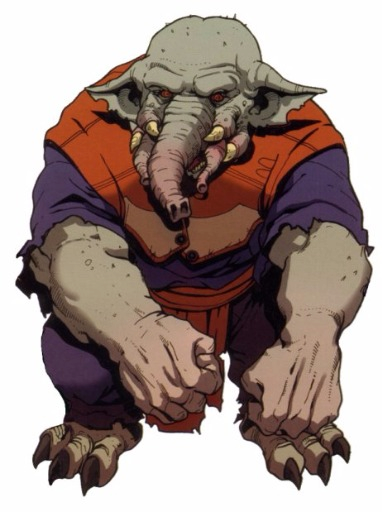
\includegraphics[width=80mm]{./content/img/meredith.png}
\begin{figure}[h]
\end{figure}
\end{center}

\noindent

The weird-noise making, portal-door-creating elephant butler of Lazarus.  Meredith's ability to conjure doorways between dimensions made her invaluable to Hell's operations, though her social skills left something to be desired, she stood up Mark on his prom night.

\smallskip

\subsection*{Trayvon}

\noindent

Trayvon was a Tengu Book Burner and colleague of Burnie prior to the great Book Burner purges.  Boasting the longest wingspan of any Book Burner to have ever held a lighter, Trayvon was a manic-depressive control freak.  Trayvon and Burnie managed to conceive a child together, the details of which remain mercifully unclear.

\smallskip

\subsection*{Ruh'Breks}

\noindent

One of the last great magic users in the world.  Ruh'Breks was an ancient, dying sorcerer who had sealed himself away in his underground tower centuries ago.  He unknowingly mentored the Goblins through the magical texts and picture books left in his tower, and was the inventor and builder of the airship that would become The Gary.  He also created the legendary Puzzle Die, a magical cube with dozens of functions including teleportation, flight, invisibility, and a wish spell on a 10,000 year cooldown.

After joining the party as ``Ruh'Breks Sensei'', he sacrificed himself protecting the airship during the assault on Masuda, holding back a giant mountain creature with his last reserves of power.  His final words: ``You must get back to Velterra.''

\smallskip

\subsection*{Arbiter Kiros}

\begin{center}
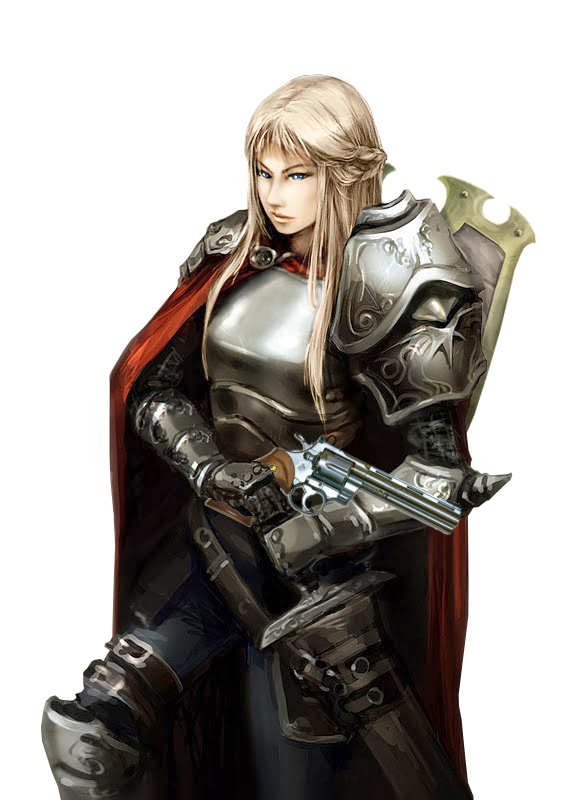
\includegraphics[width=80mm]{./content/img/kiros.png}
\begin{figure}[h]
\end{figure}
\end{center}

\noindent

Kiros is a terrifying Arbiter, a plate-armoured Church enforcer carrying a gun bigger and badder than Riphard's.  She is renowned as the first person to ever cause Kolo to soil himself.  Despite her fearsome reputation, Kiros developed a grudging respect for the party after witnessing their actions in Logarsk, where they exposed the Marshall's abuse of children in the church basement.

She likes Riphard, respects Otoria, and came around to helping the team once the Inquisition started making its presence felt.  She was good friends with ``the machine gun wielding maniac.''

After the party left Hope's Rest, Kiros was captured by the Church and replaced with a doppelganger who reported on the group's movements.  The real Kiros was taken to Seven's Spire and tortured on a rack in the prison level.  She was found barely alive by Myron, who stuffed her mouth with cured beef jerky and willed her back from the edge.  Upon revival, she immediately demanded to know the whereabouts of Arbiter Khan.  When the party encountered Khan, Kiros unloaded a full set of chambered rounds into him as he advanced towards her.

\smallskip

\subsection*{Holly}

\begin{center}
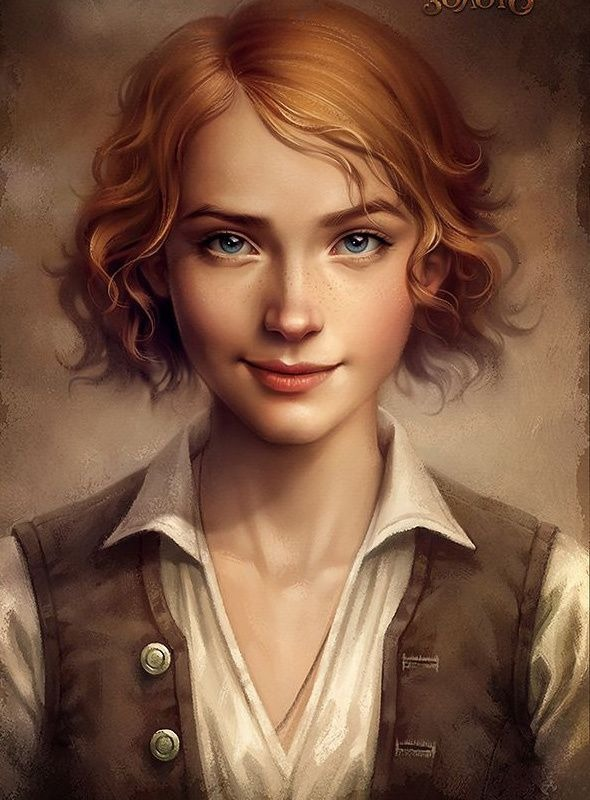
\includegraphics[width=80mm]{./content/img/holly.jpg}
\begin{figure}[h]
\end{figure}
\end{center}

\noindent

The keeper of the Tower of Imota Kan (Nakatomi backwards) in Riverfall.  Holly managed the tower's vaults, library, and social events.  She let the party in to examine the sacred artefacts and hosted them at a party where Otoria met people from her home continent.  During the Die Hard heist, Holly was taken hostage but survived thanks to the party's intervention.

\smallskip

\subsection*{Bilbo and Dildo, Riphard's Twins}

\begin{center}
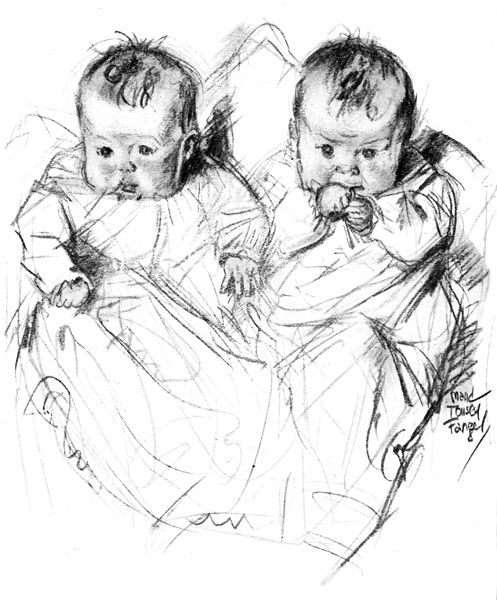
\includegraphics[width=80mm]{./content/img/twins.jpg}
\begin{figure}[h]
\end{figure}
\end{center}

\noindent

Twins born to Riphard and Delilah during the Tom'ardy Mountains expedition.  Blessed by the gods and believed to possess special powers, these children represent the next generation of the Hardstone dynasty.  Their mother was killed by Kolo shortly after their birth, and Exme stopped time to rescue them during the ensuing chaos.  After the tragedy, they were cared for by Burnie's adoptive dwarven parents Gerald and his wife, who joined the airship crew as babysitters.

\smallskip

\subsection*{Derek Bobacious}

\begin{center}
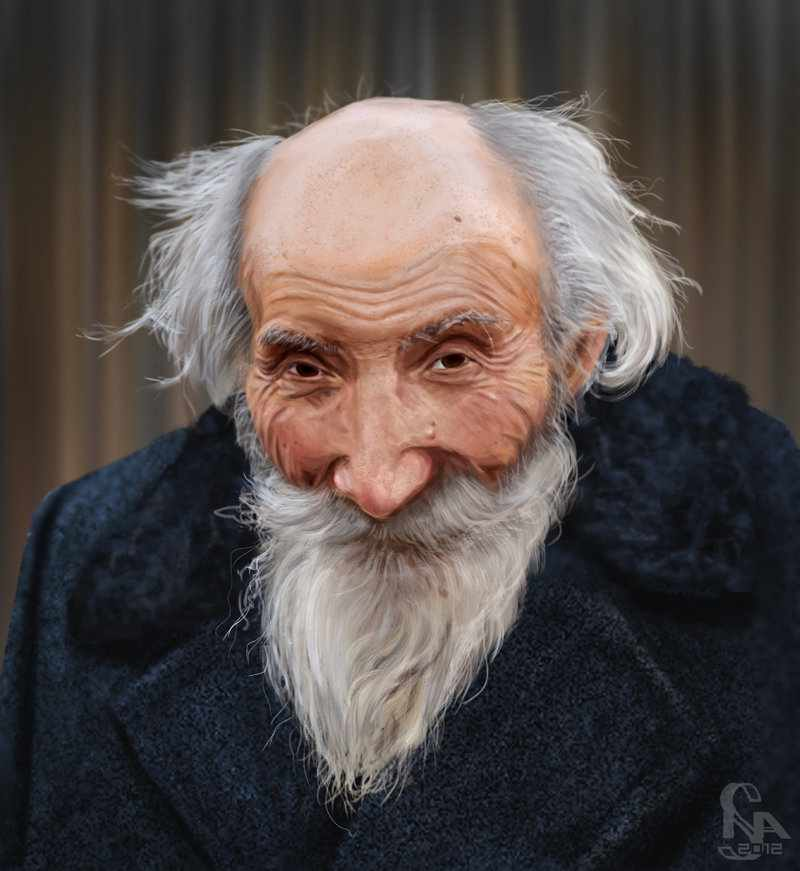
\includegraphics[width=80mm]{./content/img/derek.png}
\begin{figure}[h]
\end{figure}
\end{center}

\noindent

A discerning but ageing bachelor, whose love for his daughter is marred only by the fact she is a total bitch.  Derek owned a nice house in Riverfall that became Riphard's first bank (Northern Rock).  He was convinced that ``the gods want to run a shop in his house'' and happily agreed.

Derek later relocated to Hope's Rest to run the marketing campaign for the Guild of Banking, sporting a casual purple and yellow suit with seven-inch lapels.  His billboard campaigns, ``We Take Interest in Your Interest'', became a fixture of the city.

\smallskip

\subsection*{King Oceani}

\begin{center}
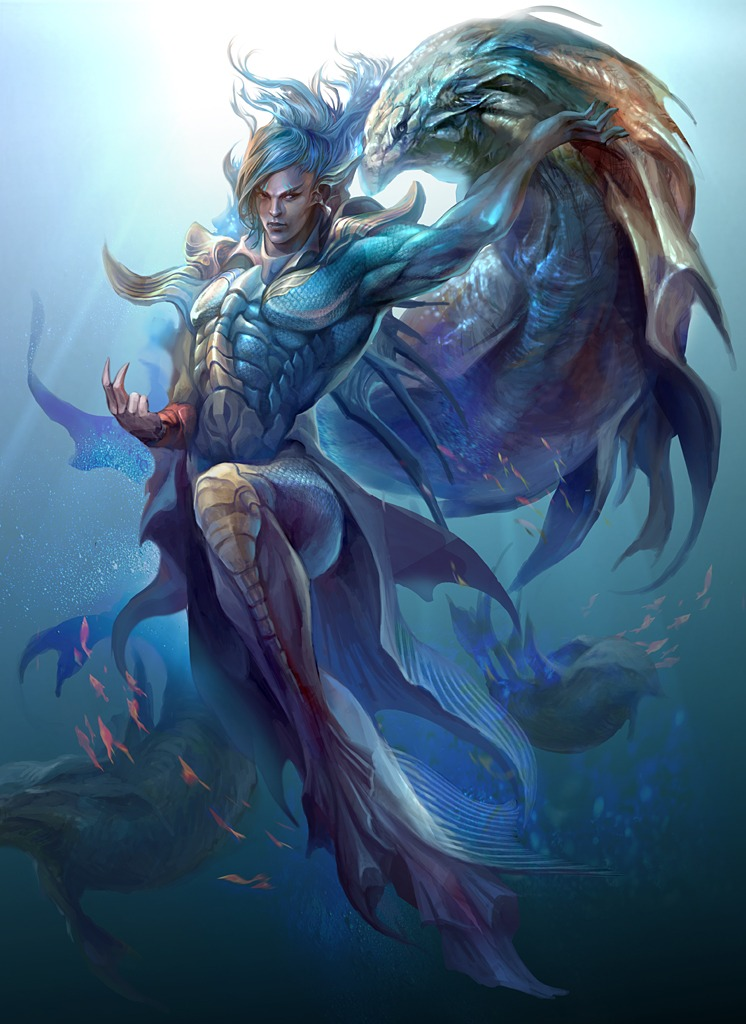
\includegraphics[width=80mm]{./content/img/kingOceani.jpg}
\begin{figure}[h]
\end{figure}
\end{center}

\noindent

Proud underwater king of the merfolk.  King Oceani (also known as O-ssu-nai) first encountered the party when they accidentally captured the head of his guard during the merfolk negotiations at New Abbergast.  Toni brokered the peace, and Oceani became a firm ally.

When the party returned to kill Acroneth the Immortal, an Aboleth terrorising the merfolk, Oceani's gratitude deepened into a committed alliance.  He fathered a child with Lady Gharbighast of New Abbergast and, when the time came, committed his entire army to the Battle of Hope's Rest.  He died during the fighting, but his ghost rallied the merfolk troops to continue the assault.  A singing fool to the end.

\smallskip

\subsection*{Tiki Tuks}

\begin{center}
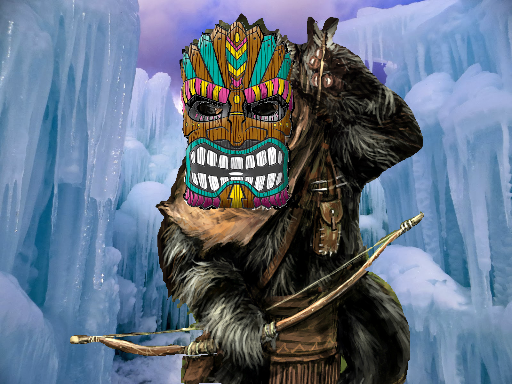
\includegraphics[width=80mm]{./content/img/tikiTuk.png}
\begin{figure}[h]
\end{figure}
\end{center}

\noindent

A race of small bear-like creatures with fearsome, culturally insensitive masks and sharp, pointed teeth.  The Tiki Tuks inhabit temples and wilderness areas throughout Velterra's southern regions and the jungles of South Africa, where cannibalistic variants were encountered.  Their war cry, ``tikki tukk doumo arigatou tikki tukk'', struck fear into the hearts of none.  Kolo could speak their language and occasionally posed as a visiting relative.

\smallskip

\subsection*{Garbigail}

\begin{center}
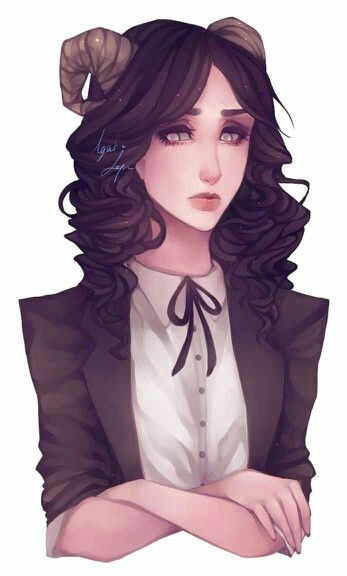
\includegraphics[width=80mm]{./content/img/arbigail.jpg}
\begin{figure}[h]
\end{figure}
\end{center}

\noindent

Garbigail, also known as Abigail, took over the Gary Guild in Hope's Rest while the party was away on the Masuda campaign.  She had survived poisoning, beaten chicken disease, and spoken to Gary in a vision, which apparently qualified her for the role.  Slightly Scouse in accent, she transformed the Garys from a loosely organised guild into a pseudo-religious peace movement, complete with Gary's original logo.

When the party returned and explained what Gary actually stood for, Garbigail agreed to fight the good fight.  The Garys answered the call for the final battle, suffering heavy casualties at the Battle of Hope's Rest in service of the ideals their founder had lived and died for.

\smallskip

\subsection*{Arbigal}

\noindent

Lazarus's boss in Hell.  Used brutal underhanded management tactics to gain control of the infernal bureaucracy.  Arbigal represents the worst of corporate politics, a creature who rose to power not through merit or strength, but through diabolical office manoeuvring of the most literal kind.

\smallskip

\subsection*{Daisuke}

\begin{center}
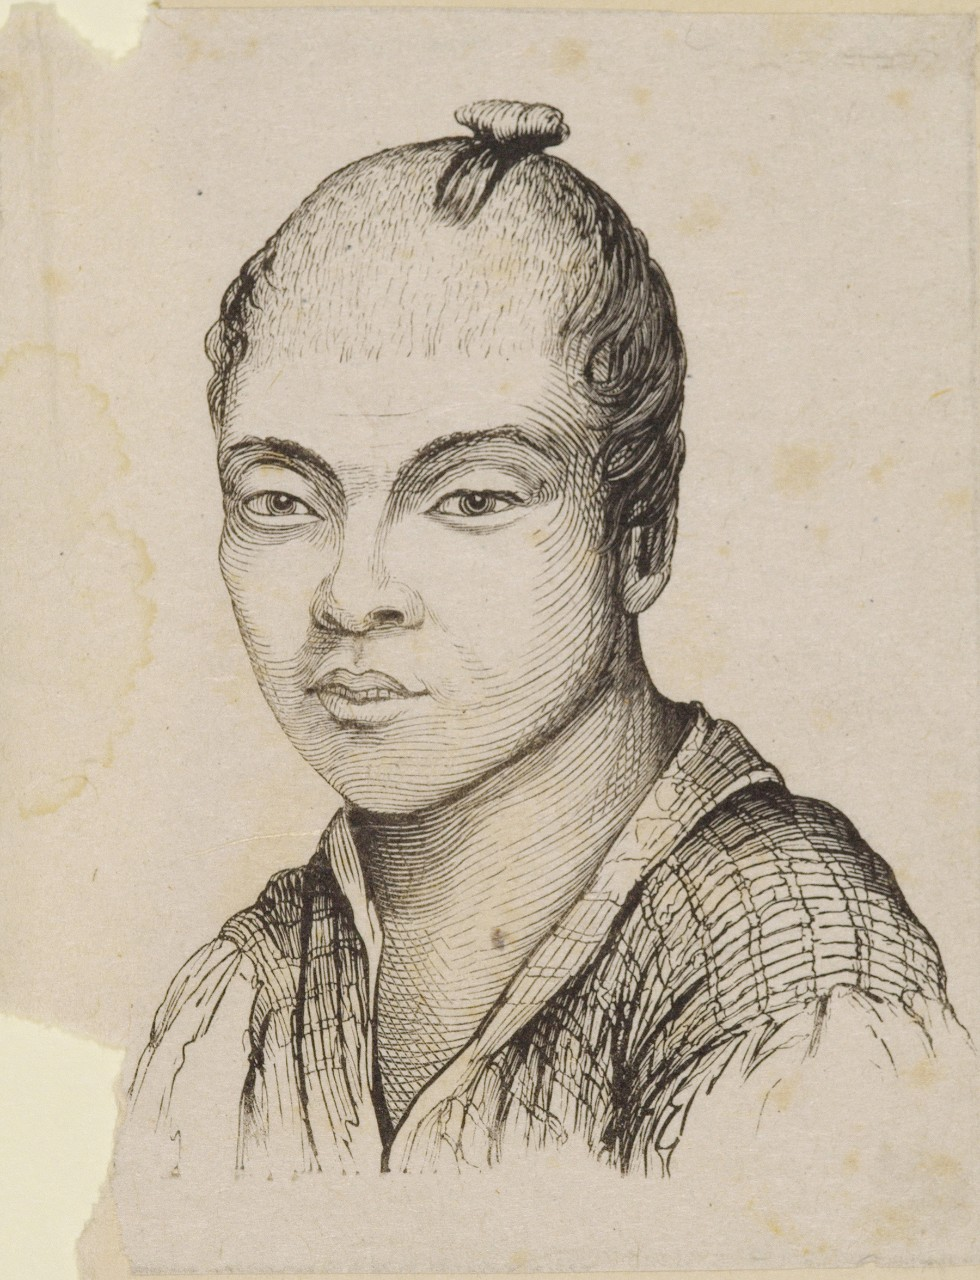
\includegraphics[width=80mm]{./content/img/daisuke.jpg}
\begin{figure}[h]
\end{figure}
\end{center}

\noindent

The party's interpreter and fixer during the Masuda campaign.  Daisuke was paid lots of money and was therefore okay doing whatever was asked of him.  He secured quotes for passage upstream, arranged boat rentals, and provided crucial cultural context, including his assessment that the local lord was ``a dick.''  A reliable, if mercenary, ally in foreign lands.

Daisuke developed a surprising romance with Archibald, the elderly librarian from the old Book Burner headquarters.  His fate was considerably less romantic, he was sacrificed by the increasingly feral Kolo to the elder entity Kalimar in the depths of the Tom'ardy mines.

\smallskip

\subsection*{Lillith}

\noindent

A half-elf Book Burner who ``actually liked Pilch'', a distinction that set her apart from most people who met him.  Lillith fled west after the great Book Burner purges and spent years in hiding before the party found her crammed into a barrel in the Tom'ardy mines.

Lillith became the group's most competent strategist.  She helped the party escape the mines when Kolo went feral, stayed behind as a dwarven diplomat after the Excalibrum cache was discovered, and convinced the Tom'ardy council to commit their forces to the alliance.  Her greatest contribution was infiltrating Seven's Spire disguised as a pastor during the Festival of Light, positioning herself inside the tower weeks before the assault.  When the party arrived in chains, it was Lillith who set them free and briefed them on the tower's layout.

She refused to be drawn into battles she considered suicidal, once sighing, overcoming her self-preservation instincts, and sliding underneath a dying Burnie to pull him from a monster's claw before informing him that she would only put herself on the line for him once, and that was it.  He reminded her that she did it really badly.

\smallskip

\subsection*{Dagenham}

\noindent

Riphard's best friend from childhood and an old dwarf of the Tom'ardy Mountains.  Dagenham was a great smithy with a dark and terrible gambling habit that Exme exploited.  His life ended in spectacular fashion when he leaned over a massive pit of centuries-old mine waste, vomited, slipped in, and was shot by Burnie for reasons that were never adequately explained.  He then sparked his tinderbox, igniting the methane and creating a ``shitty napalm'' that threw everyone backwards.  Riphard named one of the twins after him.

\smallskip

\subsection*{Google Von Maccherstein}

\noindent

Master blacksmith of Linderdorf and winner of the Blacksmith Cup alongside his partners M\"ar\"ock Gr\"unhelvem and J\"uppi Indelnacht.  The party's drunken search for Google through Linderdorf's warren of foundries and automatons became the stuff of legend.  He had gone exploring the Varg lands and had to be rescued from giants by the party before he could forge the Excalibrum weapons that would arm the group for their final assault.  His workshop in Linderdorf, staffed by the assistant Burnice and the dwarves Linus Brandler and Celina Speidel, served as the party's base of operations during the Linderdorf arc.

\smallskip

\subsection*{Buck McCraw}

\noindent

Burnie's son, originally called Trayvon Jr.  Half-human, half-Tengu, and hideously disfigured, Buck was raised by the assassin Bones after Burnie abandoned him.  He trained at the Guild of Assassins and initially attempted to kill his father before the two reconciled over a shared understanding of loss in ``a beautiful reconciliation'' where father and son ``quickly became best friends, making up for lost time.''  Buck introduced Kevin to the party as a promising PhD student needing field experience, an act of either generosity or revenge, depending on one's perspective.

\smallskip

\subsection*{Lady Gharbighast}

\noindent

Ruler of New Abbergast, the island fortress-town where the party brokered peace between the land settlers and the merfolk.  Lady Gharbighast was not a Jenny, not a merfolk, but some other kind of water person, a distinction without a difference, perhaps.  She was pregnant with King Oceani's child when the party returned to recruit her forces for the final battle.  Despite the Church's attempts to turn her against the party, she remained loyal to the alliance and committed her people to the cause.

\smallskip

\subsection*{Rolltop Kandian}

\noindent

Police chief of Hope's Rest and an old friend of Myron's.  Rolltop received Myron's warnings about the sewer killings and the Inquisitors with varying degrees of receptiveness, on one occasion responding by hitting Myron with a billy club.  In a twist that surprised no-one who had been paying attention, the epilogue of Episode 59 revealed that Rolltop himself was the serial killer stalking the city's sewers.

\smallskip

\subsection*{Lark}

\noindent

A singing swordswoman encountered during the Die Hard heist at the Tower of Imota Kan.  Lark beheaded Otoria with a katana, the group's first real loss, and one that hit hard.  Not to be confused with one of Mark O'Synne's coloured copies, also named Lark, who was considerably less lethal and more annoying.

\subsection*{Mrs Ball}

\begin{center}
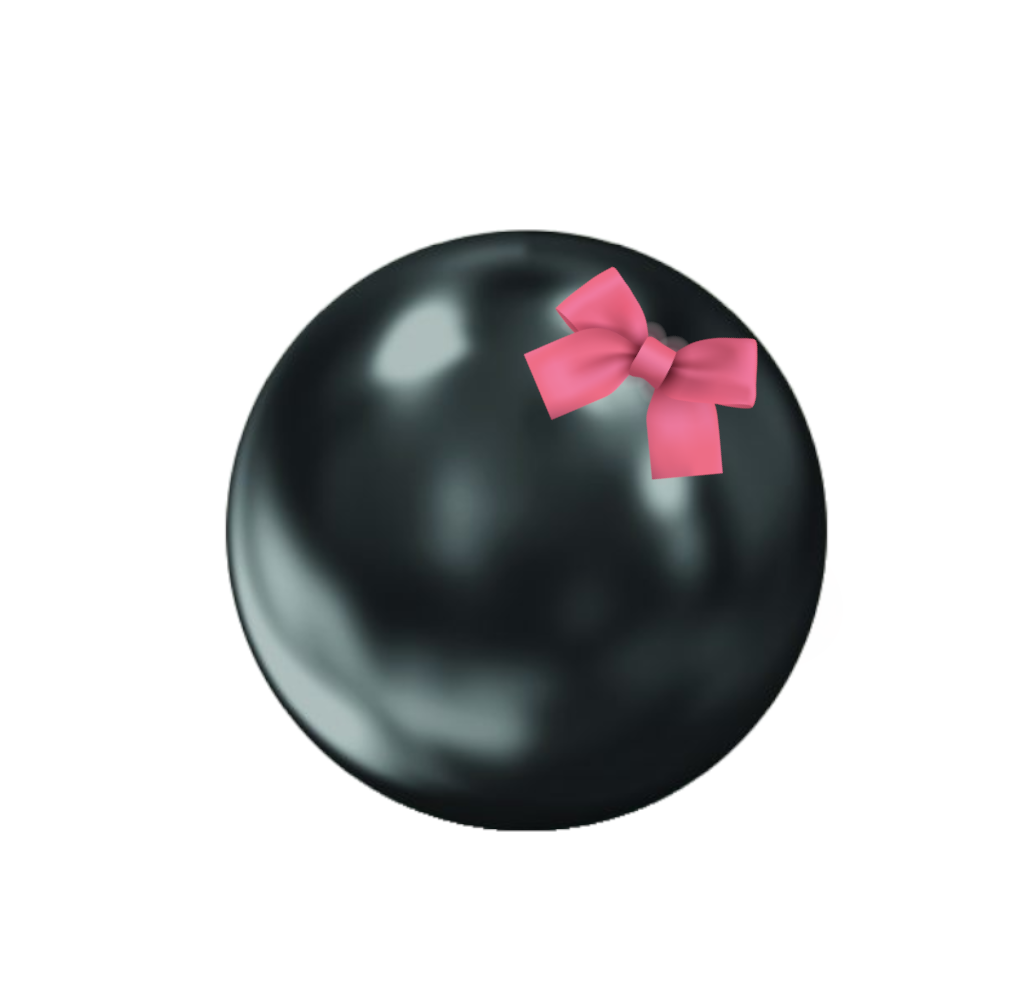
\includegraphics[width=60mm]{./content/img/MrsBall.png}\\
\textit{Mrs Ball, who contains a universe}
\end{center}

\noindent

A sentient sphere of impossibly dense metal, dressed up with an incongruous pink bow, Mrs Ball served the party in the continuation as something between a sidekick and a weapon of last resort.  She answers to a being she calls the ALLMOTHER, and her stated work is the quiet restoration of broken universes, a task glimpsed in an epilogue where she patiently rebuilds a shattered one piece by piece.

In a fight she does one thing, and does it better than anything else in the world.  When the lich Valklondar had the party beaten, Myron slammed him into Mrs Ball and the impact finished him.  Later, in the lava sanctum, with most of the party dead or dying, it was Mrs Ball who delivered her biggest ever bonk, punching clean through Kalimar, the Elder God of Creation, and killing him.  The original Mrs Ball was lost along the way, but a successor, by all accounts a more confident model, took her place.

\subsection*{David}

\noindent

A teenage tailor adopted by Myron and Exmerah, David grew up among the party's strange extended family in the years after the Spire.  He stitched the uniforms for Exme's girls' school and was, for a boy raised by a gnome Arbiter and a goblin artificer, remarkably well adjusted.  When the falling Nautiloid threatened to crush Jecede, David helped fly the airship Gary into its path to turn it aside, a piece of courage that cost the beloved airship and Captain Stick their lives but saved the city.

\subsection*{Valkar Varg}

\noindent

Warlord of a unified Varg, Valkar was the great enemy of the continuation's first half.  Where earlier Varg leaders had been brutal but mortal, Valkar made a pact with the Elder God Kalimar, brewing his goo into super-soldiers through trials that killed ninety-nine takers in a hundred.  He rode a giant eagle at the head of a hellish host of Pact warriors, and in episode 88 he announced the invasion of the south, ending any hope the party had of quietly seizing a single warband.  When Canalon descended and the war turned, Valkar fled the battlefield, and his ultimate fate was never recorded.

\subsection*{Krankle}

\noindent

A goblin alchemist with a long and ugly history, Krankle had tormented Kolo and Exmerah when they were children in the Varg.  By the time the party caught up with him he was working for Valkar, studying Kalimar's goo to engineer a controllable version called Kalimel.  Found at last in a laboratory papered with pornography, he was persuaded to switch sides for gold, protection and, in his own terms, dark-haired white women, agreeing to brew an antidote and handing over a tracker he had planted on Valkar.

\subsection*{Minor Figures from the Party's Records}

The campaign wiki recorded a host of smaller names who never earned a full page but deserve to be remembered:

\begin{DndTable}[color=PhbLightCyan]{lX}
  \textbf{Gerard the Hunter} & The Vathos Boundary hunter who gave Pilch and Otoria the information on the southern wilds. \\
  \textbf{Hans Gruber} & Full name of the mercenary leader behind the Tower of Imota Kan heist. \\
  \textbf{Diego Escobar} & Leader of ``a robbing hood'' near Vathos Boundary. ``Pretty boy got run over by horses and skewered in his own camp.'' \\
  \textbf{Henry \& Henri} & Henry: a competent dwarf who worked in Kolo's drug alchemy lab in Hope's Rest. Henri: Kolo's gabrin bin man, an ``incompetent Gabrin swine that can't even take the bins out.'' \\
  \textbf{Hestor's Caravan} & The caravan that carried the party across the land: leader Hestor; guards Leorable, Dukey, Dallius and Job; merchants Boamos, Tillie, Sabina, Maarah and Sidney. \\
  \textbf{Boa Sab} & Jungle guide who led the party to the Tikki Tukk village, only to be slaughtered in the incident. \\
  \textbf{The Tribal Leader} & Jungle tribal chief. Nice guy, hated magic, loved dancing. \\
  \textbf{Terry} & Very friendly emancipated triceratops; went off to start a new life post-incident. \\
  \textbf{Trevor} & Definitely not Terry's replacement. Currently assisting in carrying out goods, and trebuchet. \\
  \textbf{Codie} & Sentient stone servant and caretaker of the Tower of Ruh'Breks. \\
  \textbf{Arbiter Killjoy} & The Arbiter who captured Burnie and had him hung in the centre of Hope's Rest. The hanging did not take. \\
  \textbf{Martha Mayfire} & Book Burner, Burnie's lover, killed in the purge. Her old crossbow, named Martha, passed to Pilch. \\
  \textbf{Lady Haremxes} & The Masudan lady who kept Vu Dong as a pet before he joined the party. \\
\end{DndTable}

\smallskip

\clearpage
